\mysubsectionformatted{Failover}
\myparagraph{
    Prima di parlare di failover, bisogna definire 3 termini apparentemente uguali:
    \begin{tcolorbox}[colback=green!5!white, colframe=green!75!black]
        \textbf{Fault (Guasto/Difetto):} L'origine o la causa di un comportamento sbagliato
    \end{tcolorbox}

    \begin{tcolorbox}[colback=purple!5!white, colframe=purple!75!black]
        \textbf{Error (Errore):} La manifestazione di un difetto nel sistema
    \end{tcolorbox}

    \begin{tcolorbox}[colback=yellow!5!white, colframe=yellow!75!black]
        \textbf{Failure (Fallimento):} La mancata erogazione di un servizio causata da un errore
    \end{tcolorbox}
    
    \begin{tcolorbox}[colback=blue!5!white, colframe=blue!75!black]
        Per \textbf{Failover} si intende un meccanismo usato per garantire la continuità di un servizio in caso di
        un eventuale guasto o interruzione del sistema. Questo meccanismo agisce in maniera trasparente all'utente,
        simulando le operazioni del sistema principale.
    \end{tcolorbox}
    \vspace{0.1cm}
    \noindent L'obiettivo di un sistema è quello di garantire affidabilità, permettendo il \\ripristino in seguito a guasti esterni.
    La soluzione consiste nel:
    \begin{enumerate}
        \item \textbf{Rendere trasparente la locazione fisica dei dati}
        \item \textbf{Rendere il failover da remoto a locale}
        \item \textbf{Replicare parzialmente i servizi locali}
    \end{enumerate}

    \noindent Nel dettaglio, la soluzione consiste nell'usare un \textbf{Proxy} (fornito da una \\ \textit{ServicesFactory} di tipo Factory)
    in grado di gestire in maniera trasparente e sicura al client eventuali guasti, mascherando la locazione e la disponibilità dei servizi.
    Nel caso in cui un servizio dovesse essere non disponibile, il proxy effettua un failover verso un servizio secondario, senza che il client debba fare nulla.
    \\
    Altro obiettivo del Proxy è far si che realizzi delle implementazioni locali dei servizi remoti che hanno problemi, in modo
    che abbiano un comportamento semplificato e vincolato.
    \\
    Nel pratico, decidiamo di creare una cache locale di oggetti di tipo \\ \textit{ProductDescription}. In questo modo, avremo un aumento
    delle performance e dell'affidabilità.

    \newpage

    \mysubsubsectionformatted{Accesso alla cache locale}

    \begin{wrapfigure}{l}{0.5\textwidth}
        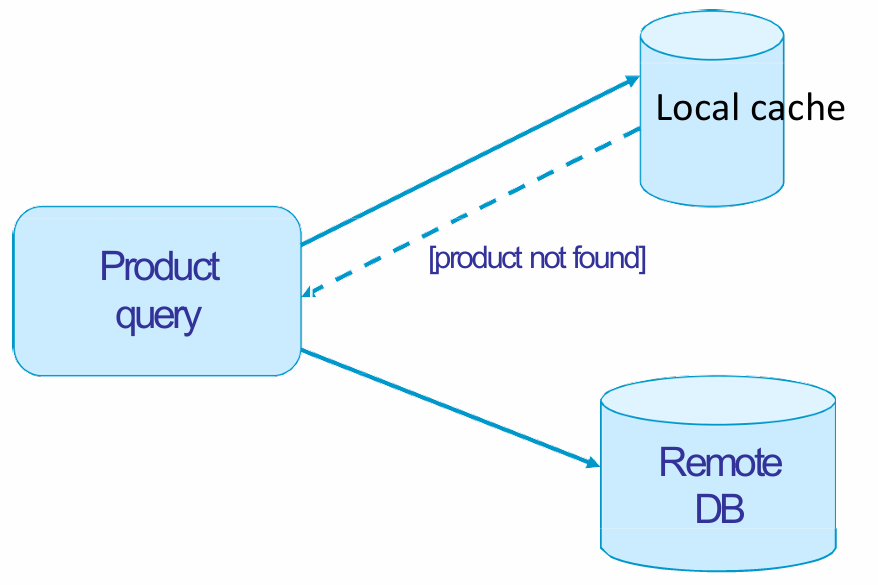
\includegraphics[scale=0.27]{Esercitazione - Design Patterns/Failover - Cache Locale.png}
    \end{wrapfigure}

    \hbadness=2000
    L'accesso alla cache locale avviene tramite il \textit{ServicesFactory}, questo ritorna un adapter a un servizio di 
    informazioni relativo ai prodotti in locale. L'adapter sarebbe l'entità che andrà a implementare le responsabilità del 
    servizio in locale, questo servizio sarà inizializzato con un riferimento verso un secondo adapter, ma quest'ultimo è 
    relativo al corrispondente servizio ma remoto.
    
    In sintesi, nel primo adapter abbiamo le responsabilità del servizio \textbf{locale}, il secondo adapter è relativo al corrispondente servizio
    locale ma in \textbf{remoto}. Se il servizio locale trova il prodotto nella cache (locale), allora lo ritorna, altrimenti inoltra la richiessta all'adapter
    del servizio remoto.
    
    Esistono due tipologie di cache:
    \begin{enumerate}
        \item Cache che mantengono in memoria una collezione di grandezza limitata ma dinamica (es. il \textit{ProductCatalog} che ha in memoria oggetti di tipo \textit{ProductDescription})
        \item Cache che mantengono in memoria una collezione più ampia di elementi su supporti persistenti (es. hard disk), questo implica che, se il sistema dovesse
        malfunzionare, la cache rimane persistente.
    \end{enumerate}

    \noindent \coloredtext[red]{Cosa succede se l'accesso alla cache locale non dà risultato e l'accesso al servizio esterno fallisce?}
    Si verificherà un \textbf{fallimento}, quindi bisogna gestirlo.
    \\
    Una soluzione comune sarebbe quella di \textbf{lanciare un'eccezione}, utile se l'errore si verifica a livello hardware. L'eccezione non deve essere percepita a 
    livello di presentazione (l'utente non deve vedere l'eccezione).
    \\
    Il pattern a cui si fa ricorso è il Design Pattern \coloredtext[blue]{\textbf{Convert Exceptions}} (descritto dopo il pattern Proxy).
    \newpage
}